% CAP2.tex

\chapter{Marco Teórico}
\label{c2} 

Este capítulo introduce los conceptos fundamentales para abordar el problema de investigación. Primero se analiza la urgencia de limitar emisiones ante el cambio climático; luego se describe el modelo original de \citeA{amigo_two_2021} identificando espacios de mejora. Se analiza también una propuesta de \citeA{munoz_lhuillier_inversion_2022} frente al problema del planificador social del modelo original. Finalmente se introduce un modelo de inatención conductual propuesto por \citeA{gabaix_behavioral_2019} el cual forma la base de la formulación propuesta para el nuevo planificador social. \medskip

\section{Capacidad Límite de las Emisiones en la Atmósfera}
Para entender el problema del cambio climático, debe considerarse que el aumento de la temperatura global está directamente relacionado con la cantidad total de dióxido de carbono que se ha emitido a la atmósfera a lo largo del tiempo. El calentamiento no depende únicamente de las emisiones de un año específico, sino de la acumulación de emisiones en el tiempo. Bajo esta idea, surge el concepto de presupuesto de gases de efecto invernadero, que en este trabajo se denominará $CAP$. Este corresponde a la cantidad total de dióxido de carbono equivalente que en Chile se puede emitir de manera consistente con el objetivo global de limitar el aumento de la temperatura media a 1,5°C, según lo establecido en el Acuerdo de París (\citeA{naciones_unidas_acuerdo_2015}) Este presupuesto funciona como un límite acumulado, lo que implica que reducir las emisiones no es suficiente para detener el calentamiento global, sino que es necesario que las emisiones netas alcancen el nivel de cero, es decir, que las emisiones generadas por la actividad humana sean compensadas por sumideros u otro mecanismo de captura. El problema radica en que la estimación exacta del $CAP$ es compleja debido a la respuesta de la naturaleza al calentamiento global y las limitaciones en la medición de los sumideros \cite{sophie_berger_francebelgium_sarah_l_connors_franceunited_kingdom_frequently_2026}. \medskip

\section{Mecanismo CAP and Trade Formulado por \protect\citeA{amigo_two_2021}}
El modelo realizado por \citeA{amigo_two_2021} propone un modelo de \textit{Cap-and-Trade} en dos etapas, donde un planificador social estima un presupuesto de emisiones en MtCO$_2$e y vende permisos cada uno correspondiente a una unidad de tCO$_2$e. Posteriormente los productores de la industria eléctrica comercializan los permisos según sus necesidades. El modelo es formulado como un problema de equilibrio estocástico de complementariedad mixta. En este, cada productor representa una tecnología específica: Solar, Eólica, Biomasa, Hidroeléctrica, Geotérmica, Carbón, Gas y Petróleo Diésel. Las tecnologías emisoras (Carbón, Gas y Petróleo Diésel) generan emisiones equivalentes a un factor de tCO$_2e/$MWh. Para operar, el sistema exige que sus emisiones sean cubiertas por la adquisición de permisos de emisión comprados previamente al ente regulador. En la primera etapa del modelo ($t=0$) el planificador social decide la cantidad total de permisos $\theta$ (tCO$_2$e) que podrán emitirse por cierto horizonte de tiempo. Los productores, a su vez, deciden su inversión en capacidad inicial con incertidumbre en la demanda que tendrán en un futuro. El modelo propone cinco escenarios equiprobables posibles para el futuro representados como $\omega \in \Omega$: demanda futura con PIB bajo (1), medio (2) y alto (4); Chile con electrificación (3)\footnote{Implica el reemplazo progresivo de combustibles por electricidad en sectores como calefacción, industria y transporte.} y de gran esfuerzo por la reducción de emisiones (5)\footnote{Supone la aplicación de políticas de eficiencia energética, lo que se traduce en una reducción significativa del consumo de electricidad en comparación con los demás escenarios.}. En la segunda etapa ($t>0$) estos redefinen su expansión en capacidad y decisiones productivas con un escenario $\omega$ ya definido. El modelo desea analizar el efecto de fijar ciertos límites de emisión dentro del sistema \textit{Cap-and-Trade} con el fin de encontrar el número de permisos que haría a Chile llegar a ser carbono neutral al 2050 y como se comporta las industrias energéticas frente a estas restricciones. \medskip

\section{El Planificador Social}
Como se mencionó previamente, el planificador social decide la cantidad de permisos denominados $\theta$, que serán emitidos para un período de tiempo $T$. Esta decisión condiciona directamente las inversiones de los generadores y los costos marginales de operación, lo que permite que el mercado eléctrico alcance un equilibrio competitivo alineado con los objetivos ambientales. La decisión de permisos a emitir debe considerar el límite ambiental real $CAP$, que al presentar incertidumbres en las mediciones, modelos y en la naturaleza, es modelado por \citeA{amigo_two_2021} como una variable aleatoria $CAP \sim \mathcal{N}(\mu,\sigma^2)$. A esto se introduce un error $\epsilon$ que controla la probabilidad de que el nivel de permisos elegido $\theta$ supere el verdadero límite ambiental $CAP$. Véase \ref{eq:probtheta}:

\begin{equation}
\label{eq:probtheta}
\Pr(\theta \ge CAP) \le \epsilon
\end{equation}

El problema a optimizar del planificador social se define como una maximización de los ingresos obtenidos por la venta de permisos ($\pi^a\cdot\theta$) menos un costo social marginal por cada $tCO_2e$, se restringe el problema a la probabilidad \ref{eq:probtheta}:

\begin{equation}
\max_{\theta} \ \theta \pi^a - \mathcal{F}(\theta)
\label{eq:objsubamigo}
\end{equation}
s.a.
\begin{equation}
\label{eq:restprobsub}
\varphi^{-1}(\epsilon)\sigma + \mu - \theta \ge 0,
\end{equation}
donde $\varphi^{-1}(\epsilon)$ corresponde a la inversa de la función de distribución acumulada de la normal estándar.

\section{El Productor}
Como se mencionó, las decisiones del planificador social afectan directamente las decisiones de producción de los generadores. Algunas tecnologías al producir energía generan emisiones contaminantes y el modelo exige que dichas emisiones sean cubiertas mediante permisos de emisión, por lo que al ser costoso emitir, el modelo busca que progresivamente las emisoras desaparezcan. Una vez que el planificador ha fijado el nivel total de permisos $\theta$ ($t>0$), los productores participan en un mercado competitivo conociendo el escenario $\omega$ y toman decisiones de expansión en capacidad ($x_i$), cantidad a producir ($Q_i$), permisos adquiridos al planificador ($A_i$), permisos comprados en el mercado secundario ($P_i$) y permisos vendidos ($V_i$). Los productores optimizan en parte, minimizando la compra de permisos $A_i$ donde la cantidad total de estos influye directamente en las restricciones de los productores: cumpliendo con que los permisos comprados sean mayores que los vendidos (\ref{eq:ventas}) y que para cada tecnología $i$ y escenario $\omega \in \Omega$ las emisiones totales generadas por la producción de electricidad no superen la cantidad de permisos de emisión disponibles (\ref{eq:emisiones}). Se resume en el Cuadro \ref{tab:variables_modelo} las principales variables y parámetros del modelo.

\begin{table}[h!]
\centering
\caption{Nomenclatura modelo \protect\citeA{amigo_two_2021}}
\label{tab:variables_modelo}
\begin{tabular}{lll}
\toprule
\textbf{Símbolo} & \textbf{Descripción} & \textbf{Unidad} \\
\midrule
$\pi^{a}$ & Precio de permisos emitidos por el planificador & USD/$tCO_2e$ \\
$\pi^{v}$ & Precio de permisos en el mercado entre productores & USD/permiso \\
$\pi^{d}$ & Precio de la electricidad pagado por el consumidor & USD/MWh \\
\midrule
$x_i$ & Inversión o expansión de capacidad del productor $i$ & MW \\
$Q_i$ & Generación eléctrica del productor $i$ & MWh \\
$A_i$ & Permisos adquiridos por el productor $i$ al planificador & $tCO_2e$\\
$P_i$ & Permisos comprados por el productor $i$ en el mercado secundario & $tCO_2e$\ \\
$V_i$ & Permisos vendidos por el productor $i$ en el mercado secundario & $tCO_2e$\ \\
$\epsilon_i$ & Factor de emisión por tecnología $i$ & $tCO_2$e/MWh \\
\midrule
$\theta$ & Permisos totales emitidos por el planificador & $tCO_2e$ \\
\bottomrule
\end{tabular}
\vspace{0.1cm}
\footnotesize{Fuente: Elaboración propia.}
\end{table}

\section{Equilibrio entre Planificador Social y Productores}
Las decisiones de los productores y el planificador se integran en un vector de equilibrio \ref{eq:equilibrio} donde los precios $\pi$ son variables endógenas resultantes de un equilibrio de mercado en el cual las decisiones de capacidad, permisos totales y la decisión del planificador congenian. 

\begin{equation}
\label{eq:equilibrio}
\left( 
\left( \pi^{d*},\, \pi^{a*},\, \pi^{v*} \right),
\, \left( x_i^{*},\, Q_i^{*},\, A_i^{*},\, P_i^{*},\, V_i^{*} \right)_{i \in \{1,\ldots,N\}},
\, \theta^{*}
\right)
\,\in\,
\pi^a\times \mathbb{X}^{N} \times \mathbb{R}_{+}
\end{equation}

El modelo integra simultáneamente tres mercados: el mercado primario de permisos, donde el planificador vende permisos a un precio $\pi^{a}$; el mercado secundario entre productores, en el cual los generadores compran y venden permisos a un precio $\pi^{v}$ y el mercado eléctrico, donde los consumidores pagan un precio $\pi^{d}$ por la energía generada.  La interacción entre estos tres mercados determina los valores de los precios y las decisiones en un equilibrio.\medskip

Las decisiones que toman los productores y el planificador social deben ser consistentes entre sí; se definen entonces, ecuaciones de equilibrio que garantizan que la decisión del planificador $\theta$ sea igual que la cantidad total de permisos $A$ en el mercado. Así mismo, la cantidad de permisos comprados entre productores debe ser igual a la cantidad vendida dentro del mercado; por último se satisface la demanda al ser igual a la cantidad de generación eléctrica ($Q_i(t,w)$). Véase la formulación:

\begin{enumerate}

    \item \textbf{Mercado secundario de permisos en $t>0$:}
    \begin{equation}
    \sum_i P_i^*(\omega) = \sum_i V_i^*(\omega) \quad \forall \omega \quad (\text{precio: } \Pi^{v*}(\omega))
    \end{equation}
    \item \textbf{Cumplimiento de demanda en $t=0$:}
    \begin{equation}
    \sum_i Q_i^*(0) = D(0) \quad (\text{precio: } \Pi^{d*}(0))
    \end{equation}
    \item \textbf{Cumplimiento de demanda en $t>0$:}
    \begin{equation}
    \sum_i Q_i^*(t,\omega) = D(t,\omega) \quad \forall t,\omega \quad (\text{precio: } \Pi^{d*}(t,\omega))
    \end{equation}
\end{enumerate}

Para los efectos de este trabajo, no se entrará en detalle del modelo completo, por lo que, para mejor comprensión se recomienda leer la sección 2 de \citeA{amigo_two_2021}.

\section{Espacio de Mejora para el Planificador Social}
\label{sec:espaciomejora}

El modelo propuesto por \citeA{amigo_two_2021} presenta oportunidades de mejora en la forma en que se modela la decisión del planificador. Si bien la formulación puede ser formalmente correcta, resulta poco realista desde el punto de vista económico ya que asume una varianza nula en la distribución normal del presupuesto de carbono ($CAP$), lo que quiere decir que en la práctica el problema se reduce a fijar determinísticamente $\theta = CAP$, valor que los autores calibran de forma exógena para representar distintos escenarios de límites en el presupuesto de emisión. Esto implica que el planificador no toma una decisión óptima basada en un criterio racional -como se esperaría de un agente económico en la práctica- sino que su acción es impuesta de manera externa al modelo.\medskip

Esta aproximación es útil para ilustrar el rango de presupuestos de emisiones bajo los cuales podría alcanzarse la carbono neutralidad hacia 2050; sin embargo, en términos de esfuerzo de decisión y comportamiento económico, resulta poco realista suponer que la cantidad óptima de permisos emitidos coincida exactamente con el $CAP$. En particular, el planificador no enfrenta un problema de maximización, sino que se limita a fijar distintos niveles de presupuesto sin una función de costos claramente definida que capture el esfuerzo o la información requerida para determinar dicho nivel. De esta forma, el modelo carece de incentivos explícitos que alineen la decisión del planificador con una elección óptima para él o el bienestar de la sociedad.
\medskip

Para ilustrar cómo la estructura de costos afecta la decisión del planificador, se analizan dos escenarios teóricos par una función de costos $F(\theta)$ que tiene el planificador: 
\begin{enumerate}
    \item Escenario con costo fijo: Se analiza un costo $F(\theta)=3$ el cual es independiente de la cantidad de permisos permitidos.
    \item Escenario con costo convexo: Se analiza una función cuadrática $F(\theta) = (\theta - 3)^2 + 1$ una parábola con vértice en (3,1) la cual si le afecta la cantidad de permisos $\theta$.
\end{enumerate}

La función de utilidad del planificador se define como $G(\theta|\pi^a,F(\theta))=\pi^a\cdot\theta-F(\theta)$. Para ambos casos mencionados, se tiene un límite $CAP$ en el eje $x=7$, un precio de venta $\pi^a=1$.

Ilustrando el primer caso en la Figura \ref{fig:ejemplo1}, se puede observar que con un $\theta<3$ el planificador tiene pérdidas en la emisión de permisos, pero pasado este punto tendrá incentivos para emitir sin restricciones llegando al valor más alto posible: $\theta^*=CAP$.

\begin{figure}[H]
    \centering
    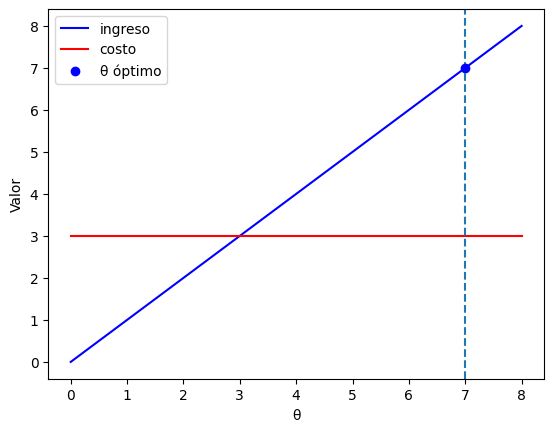
\includegraphics[width=0.7\linewidth]{ejemplo1.02.png}
    \caption{Ejemplo con F($\theta$) fijo (Fuente: elaboración propia)}
    \label{fig:ejemplo1}
\end{figure}

Para el segundo caso, si analizamos la Figura \ref{fig:ejemplo2} se puede observar que el punto $\theta=CAP$ deja de ser un óptimo. En este punto, los valores en la función objetivo del planificador queda: $7\cdot1-[(7 - 3)^2 + 1]=-10$, una utilidad negativa. Para este caso, sería preferible tomar una decisión donde $\theta$ sea igual a 2 o 5, ya que en estos puntos, si bien no se obtienen beneficios, no hay pérdidas. Entre estos dos puntos mencionados se encuentra el rango donde el planificador social tiene beneficios al emitir, con un óptimo en $\theta = 3{,}5$, lo que resulta en un beneficio dado por $G(3{,}5) = \pi^a \cdot 3{,}5 - [(3{,}5 - 3)^2 + 1] = 2{,}25$.


\begin{figure}[H]
    \centering
    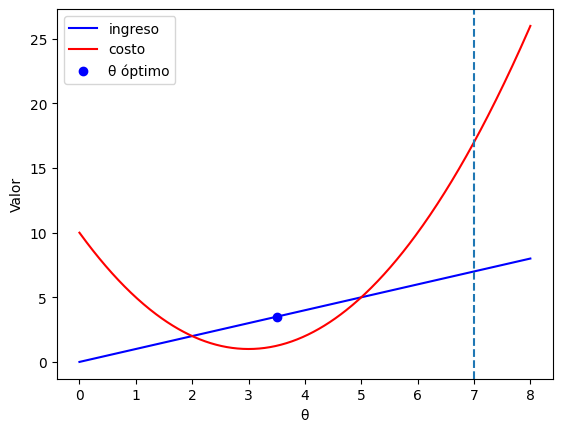
\includegraphics[width=0.7\linewidth]{ejemplo2.02.png}
    \caption{Ejemplo con F($\theta$) parabólica (Fuente: elaboración propia)}
    \label{fig:ejemplo2}
\end{figure}

Con estos ejemplos se puede observar que la falta de una definición explícita para $F(\theta)$ en el modelo original introduce una indeterminación que dificulta la obtención de un único equilibrio. Esta limitación justifica la necesidad de proponer una función de costo estructurada que capture la relación entre el límite de emisiones $\theta$ y el presupuesto de carbono $CAP$. 


\section{Precisión y Racionalidad en el planificador social}
\citeA{munoz_lhuillier_inversion_2022} propone una reformulación del modelo \citeA{amigo_two_2021}, sustituyendo el comportamiento del regulador en un marco de atención racional. Esta modificación introduce el concepto de ``ruido'' en la toma de decisiones, donde el planificador enfrenta funciones de costo que aumentan proporcionalmente a la nueva información adquirida. Para modelar este comportamiento \citeA{munoz_lhuillier_inversion_2022} involucra un parámetro $d \in [0,1]$ que representa el nivel de información pública disponible y un costo marginal $c$ asociado al procesamiento de información para mejorar el desempeño $P\in[0,1]$. \medskip

El planificador social se presenta bajo dos enfoques de optimización distintos: uno orientado al beneficio privado (Profit oriented) y el otro orientado por el bienestar  social (Welfare oriented).

\subsection{Planificador como Profit-Oriented}

En este modelo, el planificador social actúa como un agente económico que busca maximizar su beneficio neto, definido como la diferencia entre los ingresos por la venta de permisos y los costos de procesamiento de información para mejorar la precisión respecto al $CAP$. La formulación es la siguiente:

\begin{align}
\max_{\theta, P} \quad & \theta \pi^{a} P - c(P-d)^{2} \label{eq:modelo_profit_obj} \\
\text{s.a.} \quad 
& \theta \pi^{a} P - c(P-d)^{2} \geq 0 \label{eq:restriccion_participacion} \\
& \theta \leq \hat{\theta} \label{eq:restriccion_theta_hat} \\
& 0 \leq P \leq 1 \label{eq:restriccion_precio} \\
& \theta \geq 0 \label{eq:restriccion_theta}
\end{align}

Donde la restricción \ref{eq:restriccion_participacion} asegura que los ingresos del planificador no sean negativos; la restricción \ref{eq:restriccion_theta_hat} establece que los permisos $\theta$ no superen al límite ambiental percibido $\hat{\theta}$, que es igual al $CAP$; la restricción \ref{eq:restriccion_precio} ya mencionada marca el limite para $P$ y la restricción \ref{eq:restriccion_theta} que los permisos no sean negativos. La solución de este problema determina un equilibrio entre el volumen de permisos $\theta$ y el nivel de desempeño $P$.

A continuación se replica el ejercicio del punto \ref{sec:espaciomejora} utilizando una función de beneficio $G(\theta|\pi^a,F(P))= \theta \pi^aP - F(P)$, donde los ingresos se representan por $B(\theta|\pi^a)=\theta \pi^aP$ y la función de costos por $F(P)= c(P - d)^2$. El objetivo es observar el comportamiento a través de los diferentes valores de $\theta$ en cada una de las funciones. Para el análisis, se asumen los valores $\pi^a = 1$, $c = 50$, $d = 0,8$, $P=0,9$ y $CAP=\hat\theta=7$. Véase la Figura \ref{fig:gsbien}

\begin{figure}[H]
    \centering
    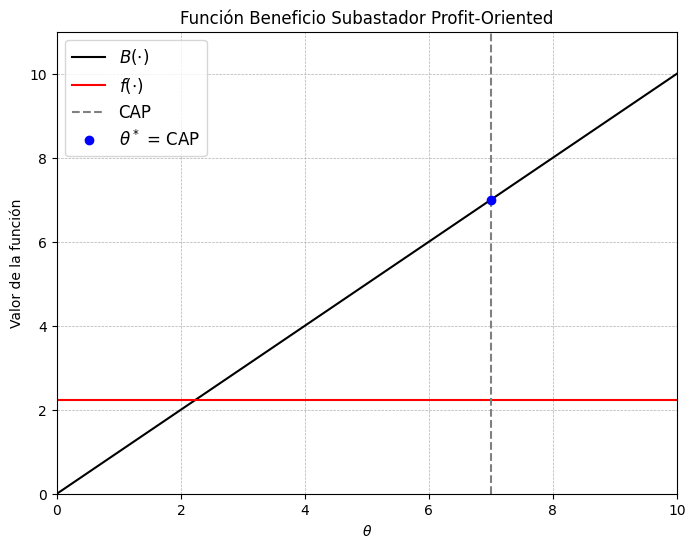
\includegraphics[width=0.7\linewidth]{planificador social profit.png}
    \caption{Función beneficio para planificador social Profit-Oriented}
    \label{fig:fporiented}
\end{figure}


Como se observa en la Figura \ref{fig:fporiented}, la función de costos toma un valor fijo, similar al comportamiento de la Figura \ref{fig:ejemplo1}. Bajo esta formulación, el modelo presenta una deficiencia estructural dado que los ingresos son linealmente crecientes respecto a $\theta$ y los costos son independientes a esta variable. Lo que es lo mismo a decir que el planificador no tiene límite económico real llegando a emitir siempre la mayor cantidad de permisos posibles, es decir, donde $\theta=CAP$. Por otro lado, la función de costos en la formulación, al no tener relación con los permisos $\theta$, resulta igual de costoso emitir un permiso a que emitir mil, lo que genera una limitación en los incentivos del modelo

\subsection{Planificador Orientado al Bienestar Social}

En este caso, el objetivo del planificador social es maximizar el bienestar colectivo. Para ello se modela la variable $P$ como:

\begin{equation}\label{eq:rendimiento}
    P(\theta \mid \hat{\theta})
    =
    1 - \frac{\lvert \theta - \hat{\theta} \rvert}{\hat{\theta}},
    \qquad
    \theta \leq 2\hat{\theta}.
\end{equation}

\medskip

La función se modela como:

\begin{align}
\max_{\theta} \quad 
& \theta \pi^{a} - c\left( P(\theta \mid \hat{\theta}) - d \right)^{2} 
\label{eq:obj_inattention} \\[6pt]
\text{s.a.} \quad 
& \theta \pi^{a} - c\left( P(\theta \mid \hat{\theta}) - d \right)^{2} \ge 0 
\label{eq:restriccion_participacion_inattention} \\[6pt]
& \theta \ge 0 
\label{eq:restriccion_theta_pos}
\end{align}


En este enfoque, el objetivo del planificador integra el desempeño $P$ como una función dependiente de $\theta$, lo que genera una relación realista sobre la emisión de permisos y el costo de procesamiento de información necesario para determinar la cantidad de permisos. Así mismo, la función objetivo (\ref{eq:obj_inattention}) busca maximizar el ingreso neto, pero ahora el costo de información está vinculado a la desviación respecto al $CAP$. La restricción \ref{eq:restriccion_participacion_inattention} asegura nuevamente que los beneficios cubran los costos operativos, mientras que la restricción \ref{eq:restriccion_theta_pos} garantiza una emisión no negativa. La diferencia clave es que, en este modelo, el planificador enfrenta una penalización económica si se aleja del presupuesto de carbono, lo que introduce un desincentivo a la emisión indiscriminada que no existía en el caso anterior.\medskip

Dicho lo anterior, se realiza el ejercicio de simulación definiendo la función de utilidad como $G(\theta) = \theta\pi^{a} - c(P(\theta \mid \hat{\theta}) - d)^{2}$, donde el ingreso corresponde a $B(\theta) = \theta\pi^{a}$ y la función de costos a $F(\theta) = c(P(\theta \mid \hat{\theta}) - d)^{2}$. Para este análisis, se asumen los mismos parámetros definidos en la sección anterior. Los resultados se presentan en la Figura \ref{fig:gsbien}.

\begin{figure}[H]
    \centering
    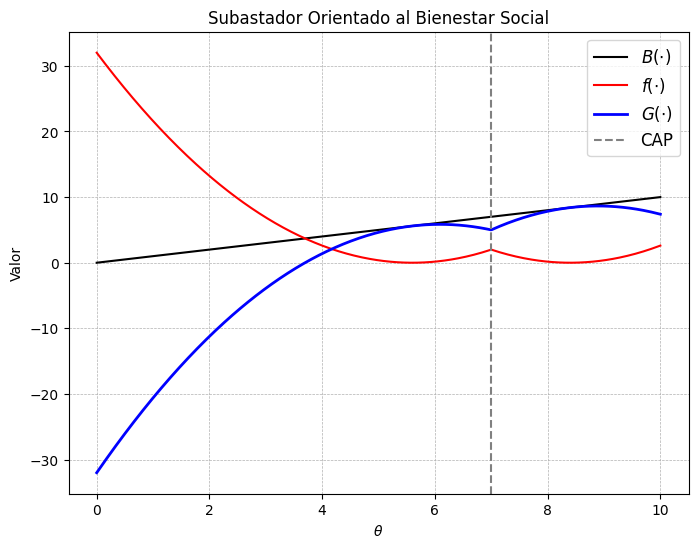
\includegraphics[width=0.7\linewidth]{planificador social bienestar.png}
    \caption{Función de Beneficios para el planificador social Orientado al Bienestar}
    \label{fig:gsbien}
\end{figure}


A diferencia del modelo anterior, bajo esta formulación sí existe un límite económico al comportamiento del planificador. Cuando $\theta = \hat{\theta} = 7$, la función de desempeño $P$ alcanza su valor máximo, lo que eleva el costo de procesamiento y reduce el beneficio neto, alejando al presupuesto de carbono de la optimalidad. Por otro lado, la función de costos presenta sus puntos mínimos en $\theta=5,6$ y $\theta=8,4$, donde el beneficio neto $G(\cdot)$ alcanza valores máximos locales. Debido a que la función de ingresos $\theta\pi^{a}$ es linealmente creciente, el óptimo global se sitúa en el punto donde el ingreso es mayor; es decir, en $\theta=8,4$. En este escenario, el planificador social optimiza su utilidad sobrepasando el $CAP$ en un $20\%$, mientras que en el segundo máximo local ($\theta=5,6$) la emisión se mantiene por debajo del límite establecido.\medskip

Bajo este escenario, surge la duda sobre qué holgura de estimación en MtCO$_2$e  es aceptable. Un nivel de permisos muy por debajo del $CAP$ compromete la producción energética nacional, mientras que uno muy por encima incrementa la contaminación. Esto sugiere que el planificador prefiere alejarse del objetivo ambiental para ahorrar en sus propios costos de gestión, en lugar de buscar el equilibrio que el país necesita. \medskip

Esto justifica una nueva formulación que permita una reducción de permisos gradual. El objetivo es una transición que no exceda los límites de contaminación ni afecte drásticamente la disponibilidad de energía, permitiendo que la baja en emisiones avance junto al aumento de la energía limpia.\medskip

\section{Modelo con Inatención Conductual}
\label{atencionconductual}
\citeA{gabaix_behavioral_2019} expone formas de modelar la atención donde explica que los tomadores de decisiones no procesan toda la información disponible como lo asume la economía racional tradicional, sino que atienden ciertos aspectos del espectro total; esto se define como inatención conductual. El autor toma como ejemplo un individuo que quiere elegir un producto del supermercado. Este individuo puede guiarse fácilmente por el precio y la calidad para la elección del producto, pero pasan desapercibidos muchos componentes como podrían ser el ingresos futuros, tipo de interés, riesgo de arrepentimiento, preferencia de otros comensales, etc. El autor recién mencionado, explica un modelo donde el comportamiento de los individuos puede ser reflejado económicamente al establecer que estos tienen una atención limitada y deciden cuánta de esa atención desean poner en las actividades que realizan, siendo coherente en que tener más atención es más costoso, en tiempo, dinero u otro. Por ejemplo, sería normal demorarse más en el supermercado si se quieren analizar más atributos sobre las compras.\medskip

\citeA{gabaix_behavioral_2019} parametriza esta atención como un valor $m$, cuando $m=1$ el individuo tiene información perfecta y cuando $m=0$ no hay atención, se dice en ese caso, que el individuo se basa en su percepción predeterminada. En la literatura, según el autor, se estima que la atención es de 0,44 en promedio, pero que es lógico que ésta sea mayor si se tienen incentivos para aumentarla.\medskip

Uno de los modelos presentados por \citeA{gabaix_behavioral_2019} describe un proceso de atención donde un agente se ``ancla'' a un valor predeterminado y luego se ajusta parcialmente al valor que desea encontrar, fenómeno conocido como anclaje y ajuste. El valor predeterminado corresponde a lo que el agente puede inferir sin atención, representado por la proporción $1-m$. El autor expresa el resultado con atención perfecta ($m=1$), como un valor verdadero existente pero no alcanzable, lo asemeja a un valor dentro de una caja negra donde todo lo que se intente obtener de ella será una señal ruidosa del valor verdadero. \medskip

Aplicando este marco teórico al modelo de \citeA{amigo_two_2021}, el valor verdadero corresponde al $CAP$, el cual sigue una distribución normal $\mathcal{N}(CAP_d,\sigma^2_{CAP})$, donde $CAP_d$ representa el valor por defecto (igual a la media) y $\sigma^2_{CAP}$ su varianza. Sin embargo, dicho valor no es observado directamente. Al intentar conocer el $CAP$, el agente únicamente percibe una señal imperfecta $CAP_s$, la cual incorpora un término de error o ruido $\epsilon$. Se define entonces:

\begin{equation}\label{eq:senal}
CAP_s = CAP + \epsilon
\end{equation}

El valor de $\epsilon$ se extrae de una distribución normal e independiente $\mathcal{N}(0, \sigma_\epsilon^2)$.

El planificador social toma la acción de emitir $\theta$ permisos y, para simplificar el análisis, su función objetivo está dada por $u(\theta,CAP)=-\frac{1}{2}(\theta-CAP)^2$, una penalización cuadrática por desviarse del $CAP$. El agente se asume racional, por lo que resolverá el problema de optimización:  $\max_{\theta} \mathbb{E}[-\frac{1}{2} (\theta-CAP)^2|CAP_s]$, obteniendo entonces, la condición de primer orden (CPO): $0=\mathbb{E}[- (\theta-CAP)|CAP_s]=\mathbb{E}[CAP|CAP_s]-\theta$. Con esto, el agente elige una acción $\theta(s)=\hat{CAP}(CAP_s)$, donde $\hat{CAP}(CAP_s)$ es el valor esperado de $CAP$ dado $CAP_s$, este valor es descrito por  \citeA{gabaix_behavioral_2019} como: 
\begin{equation}\label{eq:accion_optima}
\mathbb{E}\left[CAP|CAP_s\right] = m CAP_s+ (1 - m)CAP_d,
\end{equation}
donde
\begin{equation} \label{eq:m}
m = \frac{\sigma_{CAP}^2}{\sigma_{CAP}^2 + \sigma_\varepsilon^2}.
\end{equation}
representa el nivel de atención del agente. Este último se ancla al valor por defecto $CAP_d$ y se ajusta, mediante el grado de atención $m$, hacia la señal $CAP_s$.

Obtenemos entonces la decisión óptima del planificador social para el problema:
\begin{equation}\label{eq:theta*}
{\theta^*}(CAP_s) = m\cdot CAP_s + (1 - m)\cdot CAP_d
\end{equation}

\section{Planificador Social con Inatención Conductual}
\label{sec:planificadorIC}
Con base en el marco teórico de inatención descrito, se reformula el problema del planificador social integrando la toma de decisiones bajo inatención conductual. En esta nueva estructura, el planificador maximiza su utilidad considerando el ingreso por permisos   $\pi^a \theta$ y minimiza un costo de penalización cuadrática por desviarse del $CAP$. Se incorpora, además,  un factor marginal $\kappa$ en $USD/{tCO_2e}$ que representa el costo social de la imprecisión en la emisión respecto al $CAP$.  Un exceso de permisos incrementa la contaminación y reduce el beneficio social, mientras que una asignación insuficiente aceleraría la transición hacia tecnologías renovables en un plazo que podría superar la capacidad de adaptación del sistema eléctrico. Queda entonces la función de utilidad del nuevo planificador como:

\begin{equation}\label{eq:utilidadv}
\mathcal{V}(\theta,CAP) = \pi^a \theta - \frac{\kappa}{2}(\theta - CAP)^2.
\end{equation}

Se realiza entonces el mismo procedimiento desarrollado en la sección \ref{atencionconductual} maximizando la utilidad dada una señal $CAP_s$:

\[
\max_{\theta} \ \mathbb{E} \!\left[ \mathcal{V}(\theta,CAP)\,\big|\,CAP_s \right]
=
\max_{\theta} \ \mathbb{E}\!\left[\pi^a \theta - \frac{\kappa}{2}(\theta-CAP)^2 \,\bigg|\,CAP_s\right]
\]

Se deriva con respecto a $\theta$:
\[
0 
= \frac{\partial}{\partial \theta} 
\mathbb{E}\!\left[\pi^a \theta - \frac{\kappa}{2}(\theta-CAP)^2 \,\bigg|\,CAP_s\right]
= \mathbb{E}\!\left[\pi^a - \kappa(\theta - CAP)\,\bigg|\,CAP_s\right]
\]

Quitando de la esperanza los valores no dependientes de $CAP_s$ se obtiene la CPO:

\[
0 
= \pi^a - \kappa\,\theta + \kappa\,\mathbb{E}[CAP \mid CAP_s]
\]

Despejando la acción óptima del planificador social dada la ecuación \ref{eq:accion_optima} se tiene la decisión final \ref{eq:theta_revenue_final}:

\begin{equation}\label{eq:theta_revenue_final}
\theta^*(CAP_s) = m\,CAP_s + (1-m)\,CAP_d + \frac{\pi^a}{\kappa},
\end{equation}

Donde $m$ está definido por la ecuación \ref{eq:m}.

El término $\pi^a/\kappa$ captura el balance entre el incentivo económico a aumentar las emisiones, dado por el precio del permiso y el costo social de desviarse del presupuesto de emisiones. Mientras mayor sea $\kappa$, menor será la respuesta del planificador al precio del permiso, y viceversa.

Se resumen los parámetros en el Cuadro \ref{tab:varyparametros}.

\begin{table}[h!]
\centering
\caption{Parámetros agregados al modelo de \protect\citeA{amigo_two_2021}}
\label{tab:varyparametros}
\begin{tabular}{lll}
\hline
\textbf{Símbolo} & \textbf{Descripción} & \textbf{Unidad} \\ 
\hline
$\kappa$       & Costo social por alejarse del $CAP$         & USD/tCO$_2$e \\
$CAP_s$       & Señal observada del presupuesto de emisiones   & tCO$_2$e \\
$CAP_d$       & Presupuesto determinista del CAP               & tCO$_2$e \\
$\sigma_\epsilon^2$& Varianza del error en la señal  & tCO$_2$e \\
$\sigma_{\text{CAP}}^2$ & Varianza del CAP & tCO$_2$e \\
\hline
\end{tabular}
\end{table}

A modo de representación del modelo, se grafica la utilidad \ref{eq:utilidadv} como el ingreso y el costo en funciones separadas donde $CAP=7$, $\pi^a=1$ y $\kappa=2$. Véase la Figura \ref{fig:uvgrx}.

\begin{figure}[H]
    \centering
    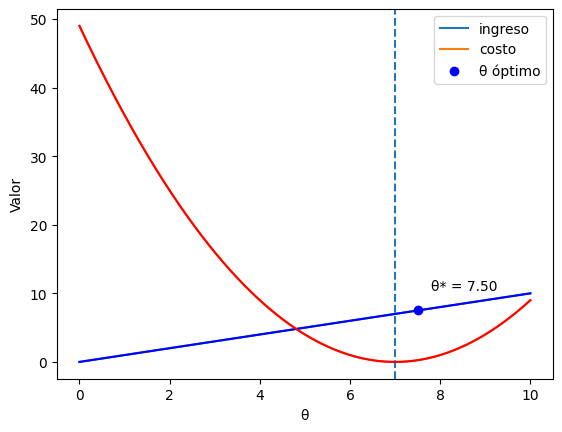
\includegraphics[width=0.75\linewidth]{vg1.png}
    \caption{Utilidad del planificador social en forma de ingreso y costo - caso $\kappa=2$ (Fuente: elaboración propia)}
    \label{fig:uvgrx}
\end{figure}

Se observa que el costo en $\theta = 0$ es cercano a 50, debido a la distancia entre el $CAP$ y el origen; a medida que la decisión se aproxima al objetivo, esta penalización disminuye. El planificador opta inicialmente por una decisión de $\theta = 7,5$ sin que el beneficio neto se vea excesivamente perjudicado, lo que sugiere que el valor de $\kappa$ permite alejarse del $CAP$ en cierto margen. Si se incrementa el factor $\kappa$ a 10, como se observa en la Figura \ref{fig:gxv2}, la decisión de permisos óptima se desplaza a $\theta = 7,1$. En este escenario, el aumento en la magnitud del costo resulta cinco veces más penalizador que en el caso anterior (nótese que ahora emitir $\theta=0$ genera un costo cercano a 250). Este incremento fuerza una decisión más cercana al objetivo y acota significativamente el espacio donde la emisión de $\theta$ produce ingresos netos, reduciendo el margen de decisión antes de incurrir en pérdidas.

\begin{figure}[H]
    \centering
    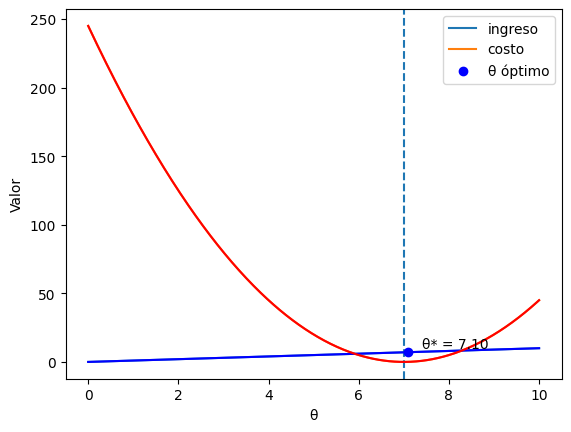
\includegraphics[width=0.75\linewidth]{vgrx.png}
    \caption{Utilidad del planificador social en forma de ingreso y costo - caso $\kappa=10$ (Fuente: elaboración propia)}
    \label{fig:gxv2}
\end{figure}









